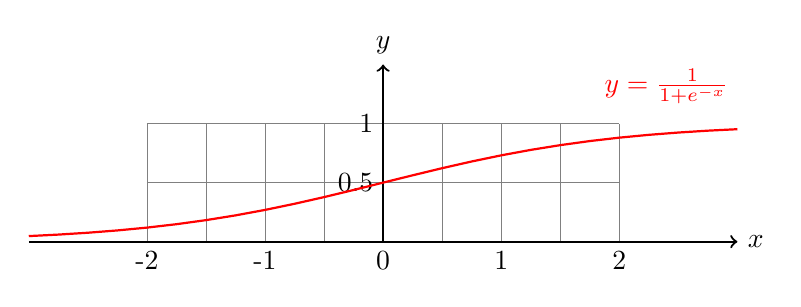
\begin{tikzpicture}[domain=-3:3, scale=1.5]
	% grid
	\draw[step=.5, very thin, color=gray] (-2, 0) grid (2, 1);
	
	% axes
	\draw[->,thick] (-3, 0) -- (3, 0) node[right] {$x$};
	\draw[->,thick] (0, 0) -- (0, 1.5) node[above] {$y$};
	\foreach \x in {-2, ..., 2}
		\node[anchor=north] at (\x, 0) {\x};
	\foreach \y in {0.5, 1}
		\node[anchor=east] at (0, \y) {\y};
		
	% sigmoid function
	\draw[thick, color=red] plot (\x, {1 / (1 + e^-\x)}) 
		node[anchor=north,  xshift=-9mm, yshift=9mm] {$y=\frac{1}{1+e^{-x}}$};
\end{tikzpicture}